
\section{Styretøj servo}

Til er kontrollere bilens styretøj er der valgt en RC servo. Skolen havde nogle Corona CS238MG \cite{Corona-CS238MG} servoer liggende på lager. Databladet var meget mangelfuld og derfor blev der søgt på Wikipedia \cite{wiki-RC-Servo} for at finde ud af hvordan de virker.

\begin{figure}[h]
	\centering
	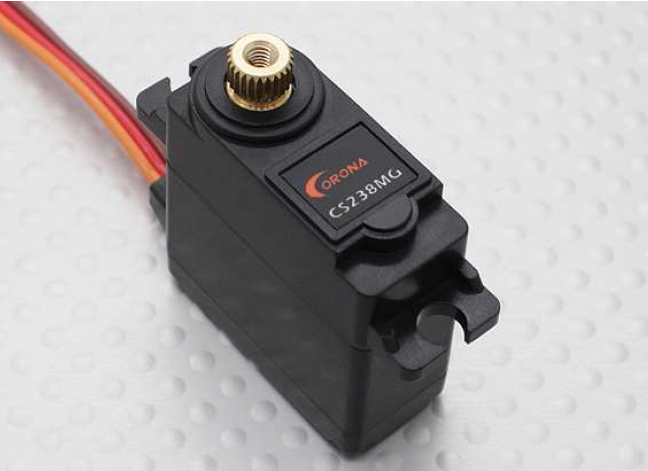
\includegraphics[width=\textwidth* 6/10]{../fig/billeder/corona_RC_Servo}
	\caption{Billed af Corona CS238MG}
	\label{fig:Corona_CS238MG}
\end{figure}  

Efter nogle tests med Analog Discovery funktionsgenerator og oscilloskop viste det sig af den kørte bedst mellem 150-200 Hz og mellem 0.5 og 2.5ms duty cycle. //
Det logiske niveau på udgangssignalerne ligger på 3.3V og servoen ligger mellem 4,8-6,0V. Det var derfor nødvendig at lave et lille print til at konvertere signalerne fra 3,3V til 5V.  

\begin{figure}[h]
	\centering
	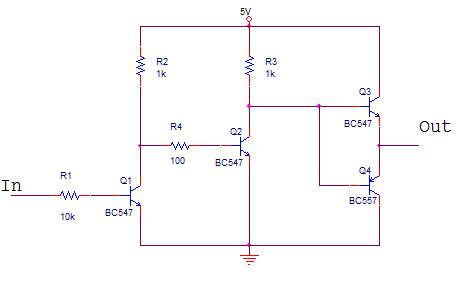
\includegraphics[width=\textwidth* 7/10]{../fig/billeder/servo_stepup}
	\caption{Diagram af signal converter}
	\label{fig:signal_converter}
\end{figure}  
